
%%%%%%%%%%%%%%%%%%%%%%%%%%%%%%%%%%%%%%%%%%%%%%%%%%%%%%%%%%%%%%%%%%%%%
%% This is a (brief) model paper using the achemso class
%% The document class accepts keyval options, which should include
%% the target journal and optionally the manuscript type.
%%%%%%%%%%%%%%%%%%%%%%%%%%%%%%%%%%%%%%%%%%%%%%%%%%%%%%%%%%%%%%%%%%%%%
\documentclass[journal=jacsat,manuscript=article]{achemso}

%%%%%%%%%%%%%%%%%%%%%%%%%%%%%%%%%%%%%%%%%%%%%%%%%%%%%%%%%%%%%%%%%%%%%
%% Place any additional packages needed here.  Only include packages
%% which are essential, to avoid problems later.
%%%%%%%%%%%%%%%%%%%%%%%%%%%%%%%%%%%%%%%%%%%%%%%%%%%%%%%%%%%%%%%%%%%%%
\usepackage{chemformula} % Formula subscripts using \ch{}
\usepackage[T1]{fontenc} % Use modern font encodings
\usepackage{lineno}
\usepackage[colorlinks = true,
            linkcolor = blue,
            urlcolor  = blue,
            citecolor = blue,
            anchorcolor = blue]{hyperref}
\usepackage{multirow}

%%%%%%%%%%%%%%%%%%%%%%%%%%%%%%%%%%%%%%%%%%%%%%%%%%%%%%%%%%%%%%%%%%%%%
%% If issues arise when submitting your manuscript, you may want to
%% un-comment the next line.  This provides information on the
%% version of every file you have used.
%%%%%%%%%%%%%%%%%%%%%%%%%%%%%%%%%%%%%%%%%%%%%%%%%%%%%%%%%%%%%%%%%%%%%
%%\listfiles

%%%%%%%%%%%%%%%%%%%%%%%%%%%%%%%%%%%%%%%%%%%%%%%%%%%%%%%%%%%%%%%%%%%%%
%% Place any additional macros here.  Please use \newcommand* where
%% possible, and avoid layout-changing macros (which are not used
%% when typesetting).
%%%%%%%%%%%%%%%%%%%%%%%%%%%%%%%%%%%%%%%%%%%%%%%%%%%%%%%%%%%%%%%%%%%%%
\newcommand*\mycommand[1]{\texttt{\emph{#1}}}

%%%%%%%%%%%%%%%%%%%%%%%%%%%%%%%%%%%%%%%%%%%%%%%%%%%%%%%%%%%%%%%%%%%%%
%% Meta-data block
%% ---------------
%% Each author should be given as a separate \author command.
%%
%% Corresponding authors should have an e-mail given after the author
%% name as an \email command. Phone and fax numbers can be given
%% using \phone and \fax, respectively; this information is optional.
%%
%% The affiliation of authors is given after the authors; each
%% \affiliation command applies to all preceding authors not already
%% assigned an affiliation.
%%
%% The affiliation takes an option argument for the short name.  This
%% will typically be something like "University of Somewhere".
%%
%% The \altaffiliation macro should be used for new address, etc.
%% On the other hand, \alsoaffiliation is used on a per author basis
%% when authors are associated with multiple institutions.
%%%%%%%%%%%%%%%%%%%%%%%%%%%%%%%%%%%%%%%%%%%%%%%%%%%%%%%%%%%%%%%%%%%%%
\author{Adriana Ipiña}
\email{ipina@ifir-conicet.gov.ar}
% \affiliation{corresponding author}
\affiliation{Instituto de Física Rosario (CONICET-UNR), Rosario, Argentina}
\alsoaffiliation{Centro de Ciencias de la Atmósfera, Universidad Nacional Autónoma de México, Mexico City, Mexico}

\author{Gamaliel López-Padilla}
\affiliation{Facultad de Ciencias Físico Matemáticas, Universidad Autónoma de Nuevo León, San Nicolás de los Garza, México}

\author{Armando Retama}
% \altaffiliation{A shared footnote}
% \email{i.k.groupleader@unknown.uu}
% \phone{+123 (0)123 4445556}
% \fax{+123 (0)123 4445557}
\affiliation{Independent researcher, Mexico City, Mexico}
% \alsoaffiliation[Second University]
% {Department of Chemistry, Second University, Nearby Town}

\author{Rubén D. Piacentini}
% \email{s.k.laborator@bigpharma.co}
\affiliation{Instituto de Física Rosario (CONICET-UNR), Rosario, Argentina}

\author{Sasha Madronich}
\affiliation{National Center for Atmospheric Research, Boulder, Colorado, USA}
% \alsoaffiliation[Second University]
% {Department of Chemistry, Second University, Nearby Town}



%%%%%%%%%%%%%%%%%%%%%%%%%%%%%%%%%%%%%%%%%%%%%%%%%%%%%%%%%%%%%%%%%%%%%
%% The document title should be given as usual. Some journals require
%% a running title from the author: this should be supplied as an
%% optional argument to \title.
%%%%%%%%%%%%%%%%%%%%%%%%%%%%%%%%%%%%%%%%%%%%%%%%%%%%%%%%%%%%%%%%%%%%%
\title[The Ultraviolet Environment]
  {The Ultraviolet Environment of a Tropical Megacity in Transition: Mexico
  City 2000-2019}

%%%%%%%%%%%%%%%%%%%%%%%%%%%%%%%%%%%%%%%%%%%%%%%%%%%%%%%%%%%%%%%%%%%%%
%% Some journals require a list of abbreviations or keywords to be
%% supplied. These should be set up here, and will be printed after
%% the title and author information, if needed.
%%%%%%%%%%%%%%%%%%%%%%%%%%%%%%%%%%%%%%%%%%%%%%%%%%%%%%%%%%%%%%%%%%%%%
\abbreviations{IR,NMR,UV}
\keywords{Ultraviolet radiation, UV~Index, Megacities, Air pollution,
Urban photochemistry}

%%%%%%%%%%%%%%%%%%%%%%%%%%%%%%%%%%%%%%%%%%%%%%%%%%%%%%%%%%%%%%%%%%%%%
%% The manuscript does not need to include \maketitle, which is
%% executed automatically.
%%%%%%%%%%%%%%%%%%%%%%%%%%%%%%%%%%%%%%%%%%%%%%%%%%%%%%%%%%%%%%%%%%%%%
\begin{document}
\linenumbers

%%%%%%%%%%%%%%%%%%%%%%%%%%%%%%%%%%%%%%%%%%%%%%%%%%%%%%%%%%%%%%%%%%%%%
%% The "tocentry" environment can be used to create an entry for the
%% graphical table of contents. It is given here as some journals
%% require that it is printed as part of the abstract page. It will
%% be automatically moved as appropriate.
%%%%%%%%%%%%%%%%%%%%%%%%%%%%%%%%%%%%%%%%%%%%%%%%%%%%%%%%%%%%%%%%%%%%%
\begin{tocentry}
  %
\includegraphics[width=9cm, height=3.5cm]{figures/Graphical_Abstract.png}
  
\includegraphics[scale=1]{figures/Graphical_Abstract.png}
  Some journals require a graphical entry for the Table of Contents.
  This should be laid out ``print ready'' so that the sizing of the
  text is correct.

  Inside the \texttt{tocentry} environment, the font used is Helvetica
  8\,pt, as required by \emph{Journal of the American Chemical
    Society}.

  The surrounding frame is 9\,cm by 3.5\,cm, which is the maximum
  permitted for  \emph{Journal of the American Chemical Society}
  graphical table of content entries. The box will not resize if the
  content is too big: instead it will overflow the edge of the box.

  This box and the associated title will always be printed on a
  separate page at the end of the document.

\end{tocentry}

%%%%%%%%%%%%%%%%%%%%%%%%%%%%%%%%%%%%%%%%%%%%%%%%%%%%%%%%%%%%%%%%%%%%%
%% The abstract environment will automatically gobble the contents
%% if an abstract is not used by the target journal.
%%%%%%%%%%%%%%%%%%%%%%%%%%%%%%%%%%%%%%%%%%%%%%%%%%%%%%%%%%%%%%%%%%%%%
\begin{abstract}
  Tropical regions experience naturally high levels of UV radiation, but
  urban pollution can reduce these levels substantially. We analyzed 20
  years of measurements of the UV Index (UVI) at several ground-level
  locations in the Mexico City Metropolitan Area and compared these with
  UVI values estimated from satellite overpasses observing ozone and
  clouds (but not local pollution). The ground-based measurements were
  systematically lower than the satellite-based estimates, by ca. 35\% in
  2000 and 20\% in 2019. Calculations with a radiative transfer model and
  observed concentrations of air pollutants explained well the difference
  between satellite- and ground-based UVI, and showed specific
  contributions from boundary layer and free trophosperic aerosols,
  O\textsubscript{3}, NO\textsubscript{2}, and SO\textsubscript{2}, in
  decreasing order of importance. Such large changes in UV radiation
  between 2000 and 2019 have important implications ranging from human
  health (skin cancer and cataract induction) to air pollution control
  (photochemical smog formation).
\end{abstract}



%%%%%%%%%%%%%%%%%%%%%%%%%%%%%%%%%%%%%%%%%%%%%%%%%%%%%%%%%%%%%%%%%%%%%
%% Start the main part of the manuscript here.
%%%%%%%%%%%%%%%%%%%%%%%%%%%%%%%%%%%%%%%%%%%%%%%%%%%%%%%%%%%%%%%%%%%%%
\section{Introduction}

Ultraviolet (UV) radiation is an important component of the urban
environment, affecting human populations directly through UV exposure of
skin and eyes~\citep{Taylor_1988,Varotsos_1997,Lucas_2019}
and less directly (but with great
impact) by driving the formation of photochemical smog, including
tropospheric ozone and other oxidants, as well as secondary aerosols
containing nitrates, sulfates, and
organics.\citep{LEIGHTON_1961,Seinfeld_1998,Finlayson_Pitts_2000}
These pollutants, along with others of primary origin commonly found in urban
atmospheres (e.g., black carbon, sulfur dioxide), can in turn scatter
and/or absorb UV radiation, alter its vertical distribution, and so
modify the photochemical rate of their own formation. Such feedback
complicates the calculation of both the UV radiation field (including at
the surface), and the evolution of photochemical smog in the urban
boundary layer.

The question of how air pollution alters the urban UV environment
(and~\emph{vice versa}) is not new, but studies have relied mostly on
numerical models \cite{Liu_1991,Sabziparvar_1998,Madronich_2011},
with relatively fewer available observations (e.g.,
\citet{McKenzie_2008}, \citet{Panicker_2009}, \citet{Palancar_2013},
reviewed by \citet{Bais_2015}). Increases in UV have been
estimated in association with decadal emission reductions, e.g. in
China,\citep{Hollaway_2019,Li_2018,Wang_2020}
and that have led to less-than-expected
reductions in photochemical smog, in part due to stronger UV
photochemistry.\citep{Wang_2019,Gao_2020,Ma_2020}
Emission reductions have also occurred
globally during the 2020 COVID-19 pandemic,\citep{Bauwens_2020,Venter_2020}
but ground-level ozone in some polluted areas has actually
increased,\citep{Shi_2020,Le_2020} due at least in part to the increased UV
radiation. Unfortunately, the observational data base of relevant UV
radiation remains rather sparse to evaluate such model-derived
hypotheses.~~

The environment of Mexico City is of particular interest for several
reasons: (1) Nearly 23 million people inhabit the Mexico City
Metropolitan Area (MCMA), and the UV environment has direct implications
for their health, both in terms of skin/eye UV exposure and~\emph{via}
photochemical smog formation. (2) As a tropical megacity, it is to some
extent representative of the situation of many others, with year-round
intense midday UV irradiance, a shallower atmosphere due to the city's
high elevation of 2240 m above sea level, and a transition toward newer
and cleaner technologies, leading to gradual improvements in air
quality. (3) Air quality within MCMA has undergone extensive scrutiny,
with a well-established monitoring network since
1986,\cite{RAMA}
numerous intensive field campaigns to study the
meteorology, emissions, and photochemistry of smog
formation,\citep{Doran_1998,Molina_2007,Molina_2010}
and numerical modeling incorporating the
evolving knowledge.\citep{Jazcilevich_2005,Tie_2007,Zhang_2009,Zavala_2020}
This extensive body of knowledge
provides the foundation for understanding our study.

Here, we analyze two decades of continuous measurements of the UV Index
at multiple locations within the MCMA, collected by the Secretariat of
the Environment (Secretaría del Medio Ambiente,
SEDEMA)\footnote{\url{https://www.sedema.cdmx.gob.mx/}} of the Mexico
City government as part of an intensive monitoring network over the
MCMA. The UV Index is defined as:

\begin{equation}
  \label{eq:UVI}
  UVI=40 \int_{250nm}^{400nm} E\left(\lambda,t\right) \cdot S_{er}(\lambda) d\lambda
\end{equation}

where~\(E(\lambda,t)\)\emph{~} is the solar spectral irradiance in
units of W ·m\textsuperscript{-2} ·nm\textsuperscript{-1}
and~\(S_{er}\left(\lambda\right)\) is the erythemal sensitivity of human
skin.\citep{who2002,Webb_2011}
Multiplication by 40 was chosen historically to
express the UVI in small integer numbers, but is otherwise
scientifically arbitrary.

The UVI is recognized by the World Health and Meteorological
Organizations (WHO and WMO) as a standardized metric of UV
radiation\cite{who2002} for global public information. An advantage
of using the UVI as (one) metric of UV radiation is that it is being
increasingly observed or calculated and disseminated, enabling more
objective comparisons among seasons and locations. The UVI observations
from Mexico City, considered here, are an important element of this
global picture.

While the UVI at the surface cannot be translated directly into
photolysis frequencies for various photo-labile molecules, the spectral
weighting of the UVI (ca. 300-320 nm) is approximately similar to that
for the photolysis of ozone to singlet oxygen atoms. Other UV
wavelengths are of course also important, e.g. for the photolysis of
nitrogen dioxide, and may be affected differently depending on the
pollutant. With these considerations and a few other caveats, UVI trends
examined here can also be used to infer accompanying trends in
photolysis frequencies and influences on photochemical smog formation.




\section{Methods}
\label{sec:methods}

\subsection{Ground-based measurements}

The Mexico City Metropolitan Area is located at 19.4°N, 99.1°W, 2240
meters above sea level (asl), surrounded by mountain ridges exceeding
5000 m asl, with complex topography and thermal inversions that inhibit
winds and favor intense air pollution.\citep{Whiteman_2000,Fast_2007,Carre_n_Sierra_2015}
Air quality
monitoring and surface meteorological measurements in the MCMA are
conducted continuously by the Automated Atmospheric Monitoring Network
(RAMA, by its Spanish acronym) of the Atmospheric Monitoring System
(SIMAT, by its Spanish acronym) of the Mexico City government. Since the
year 2000, UV radiometers (model 501-A, Solar Light Company Inc.,
Glenside, PA) detecting wavelengths between 280-400 nm have been
measuring erythemally-weighted solar radiation. The calibration of the
UV sensors was carried out annually by comparing against a
factory-calibrated reference sensor. The output voltages from the
measuring sensors were compared during at least one week against the UV
readings from the reference sensor to derive the calibration factor. New
calibration factors typically differed from the old ones by 2\% or less.
Reference sensors were also calibrated by the manufacturer and updated
periodically (between 3 to 5 years) to avoid any bias due to aging. Long
term calibration drift was avoided by the yearly re-calibrations.
Although at the beginning only a few stations were in operation and have
been changing, currently 11 stations are recording erythemal
irradiances, which are then multiplied by 40 (see
Eq.~{\ref{eq:UVI}}) to give UV Indices.
Table~{\ref{table:stations}} describes the location of
the stations where UV Index has been measured.
Figure~{\ref{fig:map}} shows how the radiometers of the
SIMAT have been distributed over MCMA, prioritizing the sites with more
density of population. Near real-time data for each station are
available on the SIMAT official
website~\url{http://www.aire.cdmx.gob.mx/default.php}. Daily maximum
values (\(UVI_{\max}\)) were extracted~from each of the stations
around solar noon from the time interval from 11:00 h-15:00 h CST
(Central Standard Time). This database~with 7305 continuous days of
measurements during the period 2000-2019 was analyzed.

\begin{table}[H]
  \centering
  \begin{tabular}{ccccc}
    \hline
    Station & Environment     & Lat (ºN) & Lon (ºW) & El (masl) \\ \hline
    CHO     & semi-urban zone & 19.27    & 98.89    & 2253      \\
    CUT     & ecological park & 19.72    & 99.20    & 2263      \\
    FAC     & urban           & 19.48    & 99.24    & 2299      \\
    HAN     & urban           & 19.42    & 99.08    & 2235      \\
    LAA     & urban           & 19.48    & 99.15    & 2255      \\
    MER     & downtown        & 19.42    & 99.12    & 2245      \\
    MON     & rural           & 19.46    & 98.90    & 2252      \\
    MPA     & rural           & 19.18    & 98.99    & 2594      \\
    PED     & residential     & 19.33    & 99.20    & 2326      \\
    SAG     & urban           & 19.53    & 99.03    & 2241      \\
    SFE     & residential     & 19.36    & 99.26    & 2599      \\
    TLA     & urban           & 19.53    & 99.20    & 2311      \\
    UNAM    & University city & 19.33    & 99.18    & 2294      \\\hline
  \end{tabular}
  \caption{{{{SIMAT stations, environmental descriptors and geographical
                positions. Abbreviations names: Chalco (CHA), Cuautitlán (CUT), FES Acatlán
                (FAC), Hangares (HAN), Laboratorio de Análisis Ambiental (LAA), Merced
                (MER), Montecillo (MON), Milpa Alta (MPA), Pedregal (PED), San Agustín
                (SAG), Santa Fe (SFE), National Autonomous University of Mexico (UNAM) and
                Tlalnepantla (TLA). }}}}
  \label{table:stations}
\end{table}

\begin{figure}[H]
  \begin{center}
    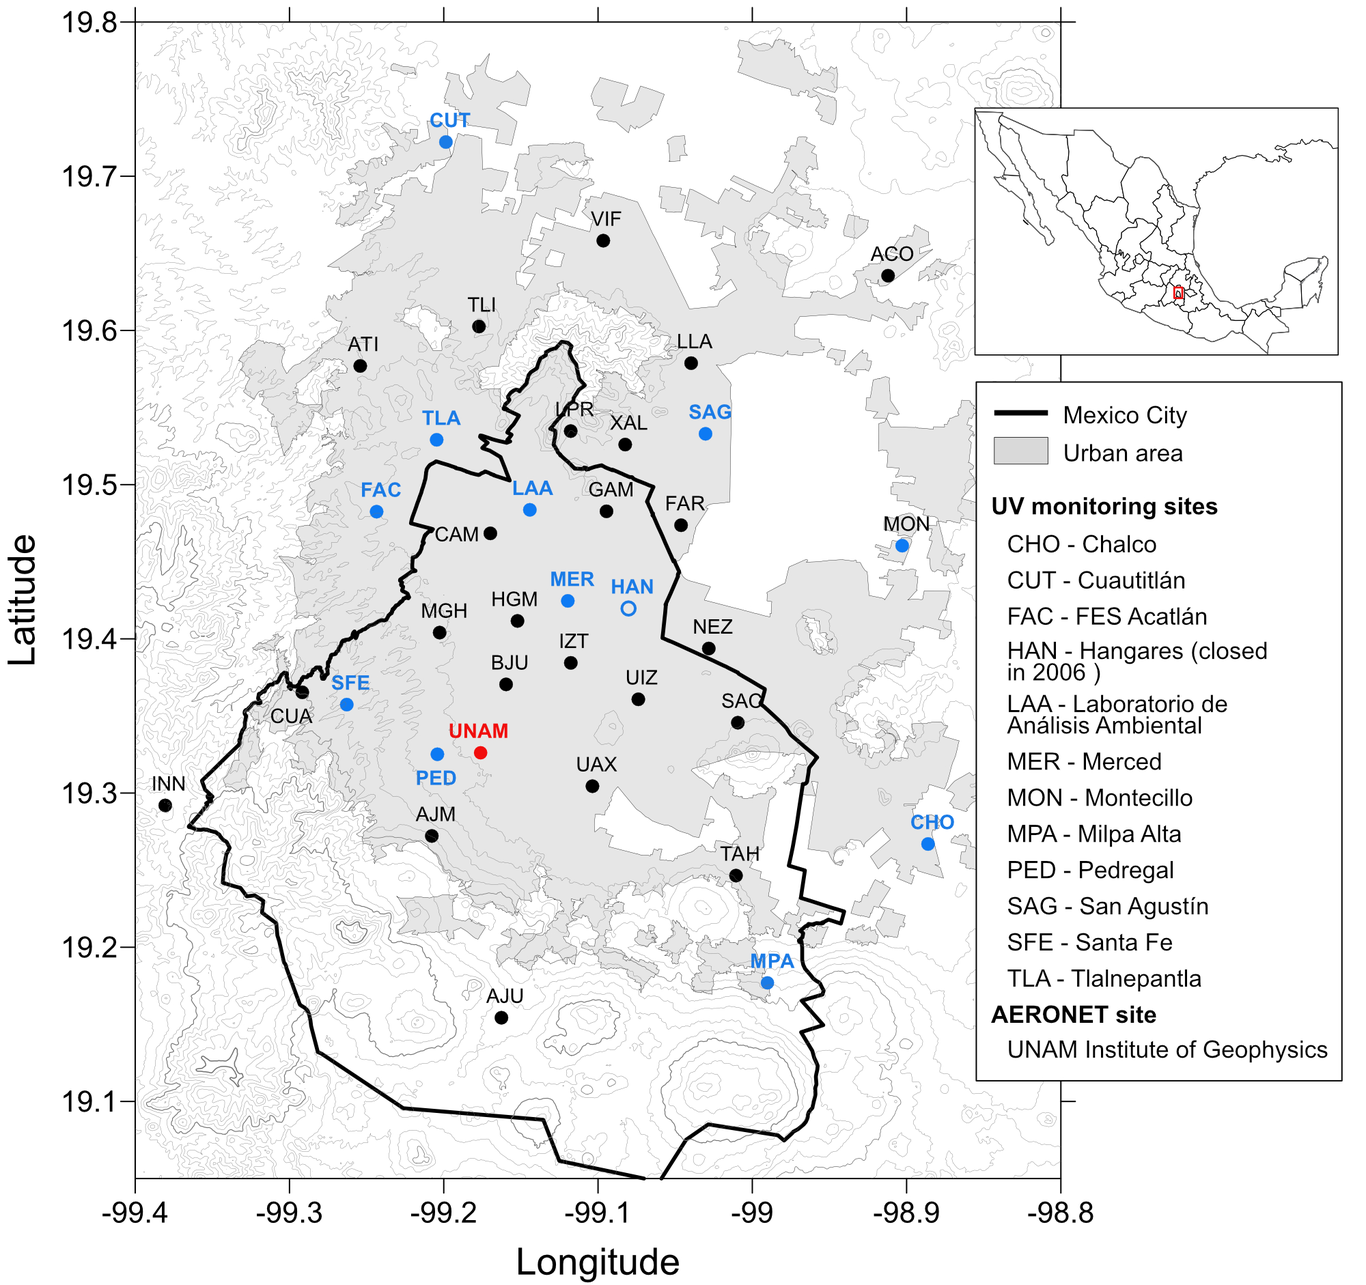
\includegraphics[width=0.70\columnwidth]{figures/map}
    \caption{{Map with the location of the SIMAT continuous monitoring stations over
          MCMA. Sites denoted by the blue solid dots correspond to SIMAT stations
          with UV measurements, while the black dots indicate SIMAT stations
          without UV measurements, the site on open blue dot represents a
          discontinued site, the red dot corresponds to the location of the
          AERONET site. The location~of Mexico City and the acronyms of the UV and
          AERONET site are shown at the upper and lower frames at the right
          respectively.
            {\label{fig:map}}%
        }}
  \end{center}
\end{figure}

With the aim to explore the relationship between UVI and air pollutants
levels, the hourly averages for ozone (O\textsubscript{3}), carbon
monoxide (CO), nitrogen dioxide (NO\textsubscript{2}), sulfur
dioxide~(SO\textsubscript{2}) and particle matter with diameter
sizes~\(\le\) 10 ~$\mu$m (PM\textsubscript{10}), were downloaded
from the SIMAT.\cite{atmosfrico} For purposes of assessing the
influence on the UV Index at solar noon, only values obtained between
11h and 15h CST were considered for the trends analysis. Pollutant
measurements are conducted by the SIMAT using regulatory-grade
commercial instruments. Measurement principles include ultraviolet
photometry (model 400E, Teledyne-API) for O\textsubscript{3},
chemiluminescence (model 200E, Teledyne-API) for NO\textsubscript{2}, UV
fluorescence (model 100E, Teledyne API) for SO\textsubscript{2}, and
infrared absorption (model 300E, Teledyne-API) for CO. The
PM\textsubscript{10} continuous mass concentration was measured with
Tapered Element Oscillating Microbalance (TEOM 1400AB or TEOM 1405 DF,
Thermo Scientific) monitors. Gaseous pollutant levels are reported in
ppb concentration units for O\textsubscript{3}, SO\textsubscript{2} and
NO\textsubscript{2}, and in ppm for CO. Particulate matter mass
concentration is reported in $\mu$g m\textsuperscript{-3} at local
conditions for temperature and pressure.

Aerosol optical depth at 340 nm was obtained from the Institute of
Geophysics of the National Autonomous University of Mexico (UNAM);
measurements were conducted with a CIMEL sun photometer model CE-318,
which is an automatic sun-sky-scanning spectral radiometer of
the AErosol RObotic NETwork (AERONET~\citep{Holben_1998}). The data
Product Level 2.0 and 1.5 (only in 2019) were selected, and annual
averages AOD\textsubscript{340} were calculated from continuous
measurements during at least 7 months. A previous study of the AOD
behavior from 2000 to 2014 demonstrated that the gaps of data did not
significantly change the trends over the analyzed
period.\citep{Carabali_2017} From 2014 to 2019 there was only 8\% of the
missing data, when the instrument was sent for calibration in 2018.


\subsection{Satellite data}

Estimates of the UV Index from satellite-based measurements of clouds
and O\textsubscript{3} were used for comparing to the ground-based
measurements. These data were provided by the Ozone Monitoring
Instrument (OMI)~on board of AURA-NASA satellite.\citep{dcio} OMI
was created in cooperation between the Netherlands Agency for Aerospace
Programmes (NIVR), the Finnish Meteorological Institute (FMI) and NASA.
OMI (hereafter OMI-Aura/NIVR-FMI-NASA) performs observations over a
geographical dimension of 13$\times$24km\textsuperscript{2} at nadir. For
Mexico City, the satellite overpass time is between 19:00h - 21:00h UTC
and data are specific for the coordinates and elevation of Mexico City.
Measurements of the ozone profile and cloud cover are used via a
radiative transfer model to estimate the UVI at the ground. The OMI web
site reports UVI values for both the overpass time, and corrected to
local solar noon.

While the early OMI estimates of the UVI did not consider aerosols in
the boundary layer, \citet{Arola_2009} suggested correcting
the clean-skies UV index with a reduction factor based on a monthly
global climatology of BL aerosols. For Mexico City a reduction of about
8\% is applied, starting ca. 2013, to the OMI UVI data.


\subsection{TUV model}

Calculations of the UV Index were also made with the Tropospheric
Ultraviolet Visible (TUV v5.3) model.\citep{Madronich_1987} The
model atmosphere was represented by 80 vertical layers, each 1 km thick,
starting at the 2.24 km asl elevation of MCMA, and for which the first
three km constitute the atmospheric boundary layer
(BL).\citep{Shaw_2007} The ozone profile above the BL is from the US
Standard Atmosphere, but rescaled to a value of 259.6 DU. Totals
including the BL contributions (of 13.7 DU in the year 2000 and 9.8 DU
in 2019, see below) were 273.1 DU in 2000 and 269.2 DU. The
climatological O\textsubscript{3} column for this latitude and season is
about 270 DU (plus or minus ca. 5 DU) so in good agreement with the
values used here.

Pollutants within the BL (including O\textsubscript{3}) are assumed to
be well mixed, in agreement with observations from the MILAGRO field
campaign that showed the disappearance of vertical gradients in the
profiles of gases \citep{Velasco_2008,Greenberg_2009} and aerosols
\citep{Rogers_2009,Lewandowski_2010} by late morning. The UV-absorbing gases
considered here are O\textsubscript{3}, NO\textsubscript{2},
and SO\textsubscript{2}, specified in ppb.

BL aerosols are modeled by prescribing the AOD at 340 nm (from AERONET
observations), scaled to other wavelengths inversely with wavelength
(Angstrom coefficient = 1.0), asymmetry factor of 0.7, and a single
scattering albedo of 0.85 at UV wavelengths, following the
determinations made in Mexico City by \citet{Corr_2009} and
\citet{Palancar_2013}.

Above the atmospheric boundary layer, the model was taken to be free of
aerosols, NO\textsubscript{2}, or SO\textsubscript{2}. In one
sensitivity study, a total AOD of 0.7 was redistributed placing 0.2 in
the free troposphere (decreasing vertically with an exponential scale
height of 4 km, and 0.5 remaining in the BL). The calculated UVI
differed by less than 1\%. Thus, as long as the total AOD is known,
knowledge of the exact vertical aerosol profile is not critical towards
ground-level UVI -- but would obviously affect the vertical structure of
photolysis frequencies.

Radiative transfer calculations were carried out with the
pseudo-spherical 4-stream option, at 1 nm steps between 280 and 400 nm.




\section{Results and Discussion}
\label{results-and-discussion}

Figure~{\ref{628947}} shows the diurnal variation of
the UVI for several specific cloud-free days, for different seasons and
several locations (CHO, MER, MON, PED, SAG, SFE and TLA). UV Index from
TUV model was used as reference of the behavior under clear sky days.
According to the comparison of measurements minute by minute, the dates
with prolonged fluctuations along the day were discarded. However,
during the rainy period (from June to October) at least a brief clouds
presence is common, as shown at CHO station around noon in 13 June
2017. Peak values range from 8 during autumn/winter to above 12
in spring/summer, in correspondence to the respective December and June
solstices. Although the stations are all within a 25 km radius,
substantial differences among them are notable. Survey of the locations
revealed that shadowing from nearby structures is not an issue. The good
agreement in the morning, followed by more divergence in the afternoon,
is consistent with the development of photo-chemical pollution hotspots
during the day. Previous studies (e.g., \citet{Castro_2001} and
\citet{Palancar_2013}) have shown
that surface UV radiation in Mexico City is attenuated significantly by
aerosols. The measurements shown in Fig.~{\ref{628947}}
are consistent with this increasing pollution during the course of the
day, with highest aerosol loading (and highest variability) attained in
the afternoon. Further support for the role of pollution in suppressing
the UVI comes from the observation made at the Santa Fe (SFE) site which
in Fig.~{\ref{628947}} are seen to be systematically
higher, e.g. by over 10\% in autumn afternoons, compared to the other
stations. The SFE station is displaced to the west from the majority of
the other stations, and remains in the outskirts. This site is also
approximately 300 m higher than Mexico City downtown, so that the
cleaner atmosphere results from both vertical and horizontal variations
in pollution levels.\citep{SEDEMA2018a} It is indeed expected to have
higher values of the UVI, in agreement with the observations.

\begin{figure}[H]
  \begin{center}
    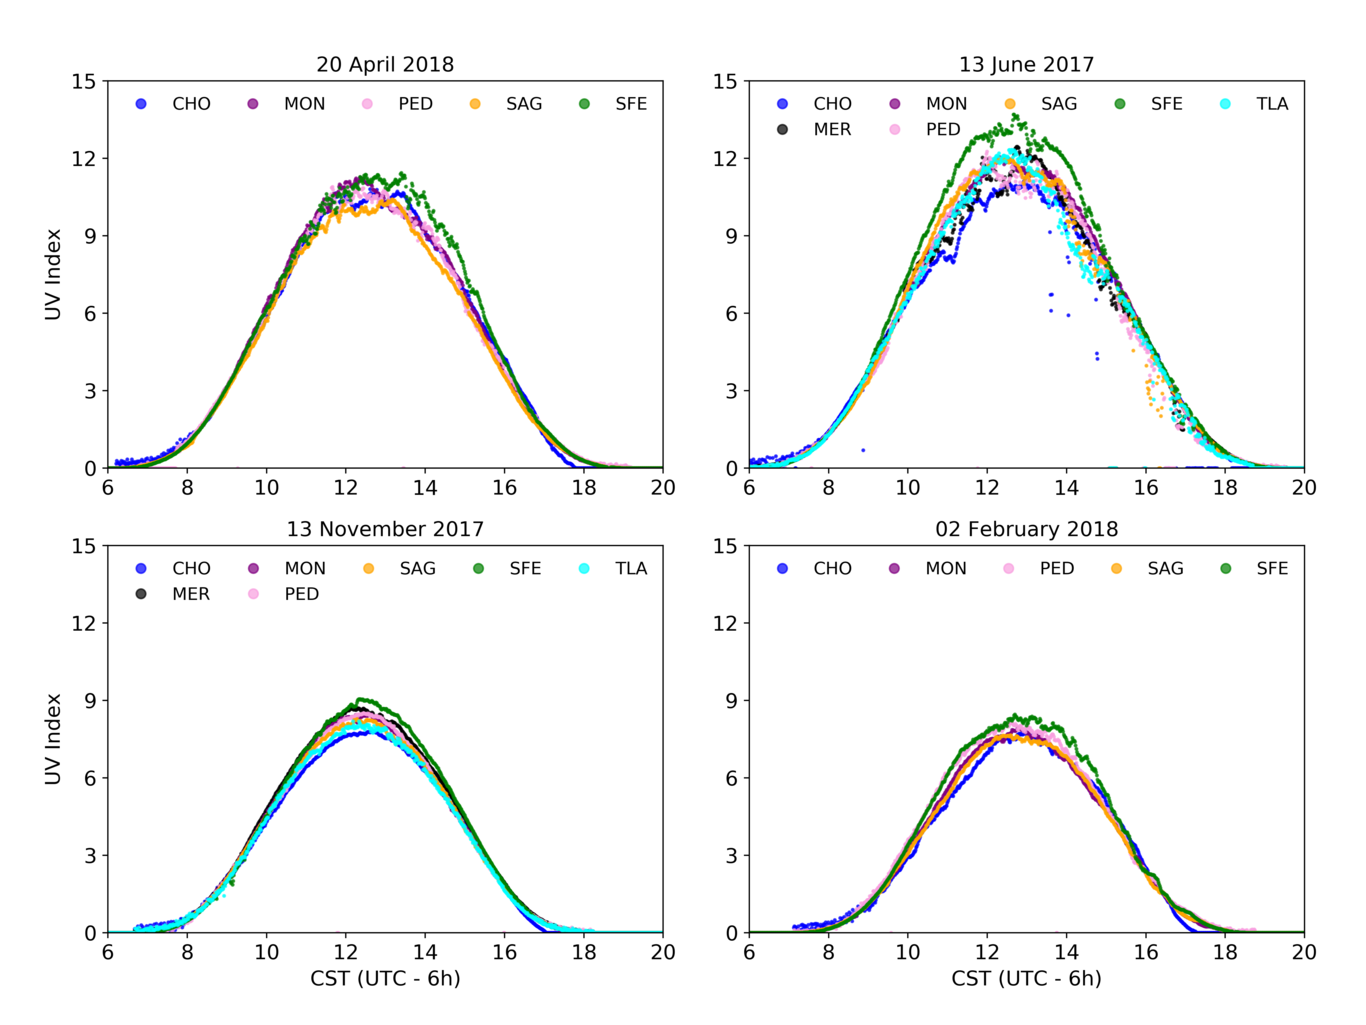
\includegraphics[width=0.70\columnwidth]{figures/season}
    \caption{{UV Index measured over MCMA by SIMAT stations each minute along the day
          under practically cloudless conditions for representative days of the
          year.
            {\label{628947}}%
        }}
  \end{center}
\end{figure}

The daily maximum UV Index of each station is denoted
by~\(UVI_{\max}\), all of them were counted in the period 2000-2019.
As shown in Figure~{\ref{461017}}, these values ranged
from 1 to 16, with a majority (61\%) of the days
experienced~\(UVI_{\max}\) values between 6 and 10, and remarkably
few, less than 1\%, in the higher 13-16 range.~The lowest values are
likely due to winter days with heavy cloud cover and low sun angles, and
UV attenuation by pollutants could also be amplified under such
conditions, due to longer photon path lengths at low sun and within
clouds. The extreme sparsity of high UVI values remains surprising, and
may be an indication of the rarity of extremely unpolluted days within
the city.

\begin{figure}[H]
  \begin{center}
    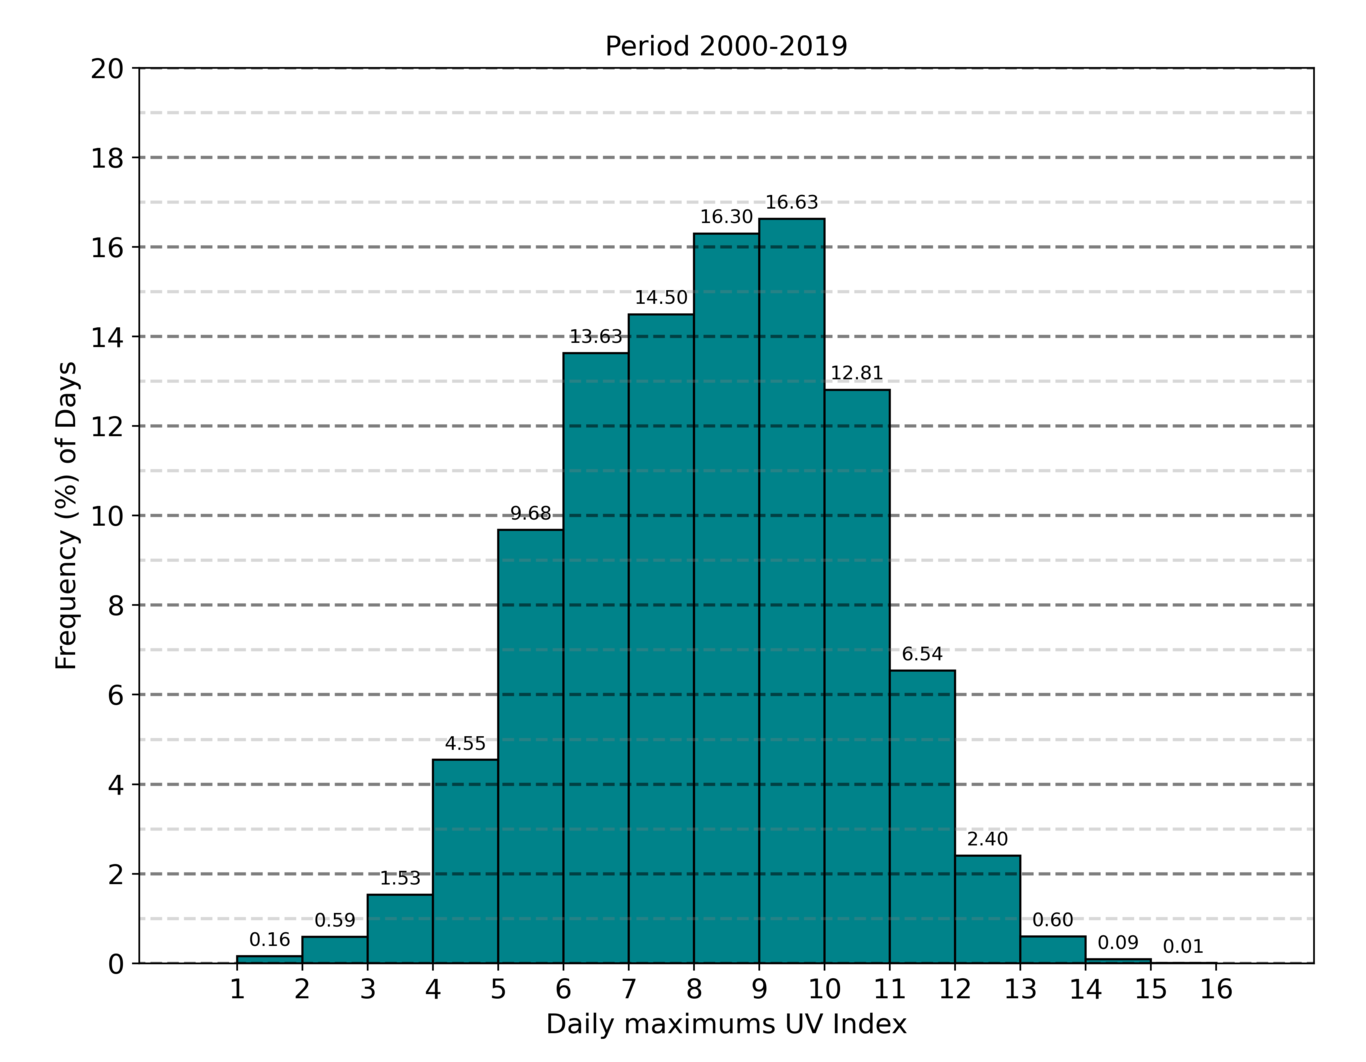
\includegraphics[width=0.49\columnwidth]{figures/Histogram}
    \caption{{Frequency distribution of daily maximums UV Index values in Mexico City
    during 2000 -2019.
    {\label{461017}}%
    }}
  \end{center}
\end{figure}

Similar patterns are found when considering the monthly average of
the~\(UVI_{\max}\)~values as shown in
Figure~{\ref{310112}}. The long-term averages present a
seasonal variation (as in Fig.~{\ref{628947}}) that
follows approximately the cosine of the noontime solar zenith angle.
Notably, values rarely if ever exceed 12 (as in
Fig.~{\ref{461017}}). The lowest average UVI (near 7)
take place in winter while from March to August the values seem to be
flattened in the range 10-11. The rather low monthly UV Index values,
mainly could be a consequence of the presence of clouds in the rainy
season. However, urban aerosol pollution sources, biomass burning for
agriculture and wood cooking also contribute to poor air quality between
March-May~\citep{Retama_2015}. Using the
maximum~\(UVI_{\max}\) from all of stations every day (one daily
point), the monthly averages (\(\overline{UVI}_m\)) were calculated along
the period 2000-2019. Long term trends in~\(\overline{UVI}_m\) are shown
in Figure~{\ref{185758}}. A clear~upward trend is seen,
with a slope for the linear fit of 0.9\%/year or +1.5 UVI units over the
two decades.


\begin{figure}[H]
  \begin{center}
    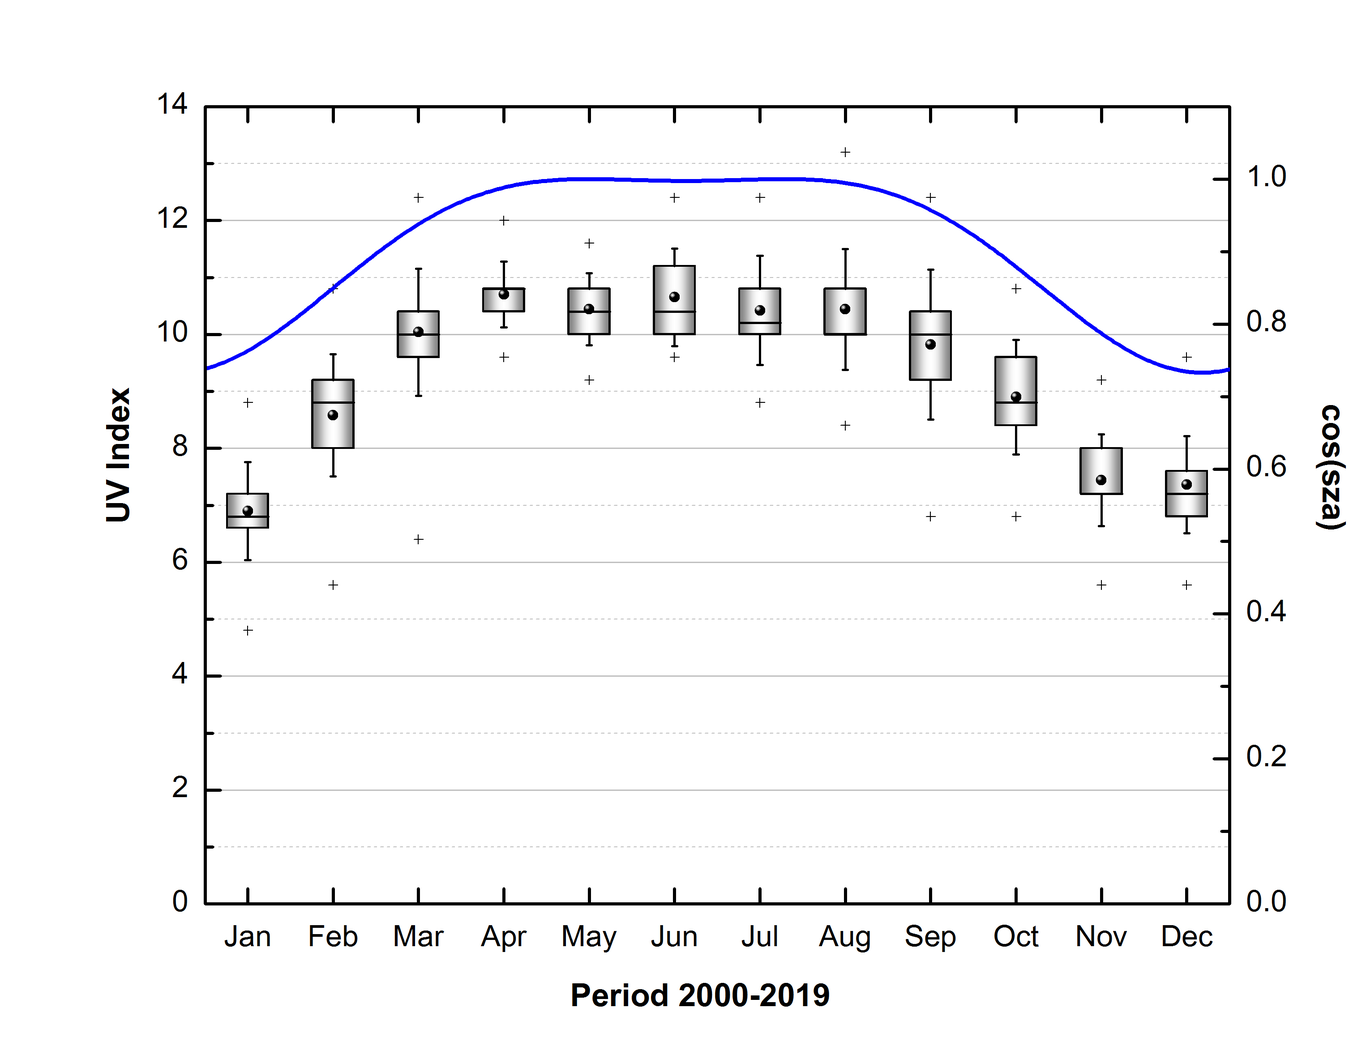
\includegraphics[width=0.70\columnwidth]{figures/Boxplotcos}
    \caption{{Boxplot of the monthly averages of the maximum UV Index values~(black
          dot) in MCMA for the period 2000-2019: median (central bold line),
          25\textsuperscript{th} and 75\textsuperscript{th} percentiles (box
          edges), standard deviation (the whiskers), the minimum and maximum
          values (plus sign) and the cosine of the solar zenith angle at solar
          noon (blue curve).
            {\label{310112}}%
        }}
  \end{center}
\end{figure}

\begin{figure}[H]
  \begin{center}
    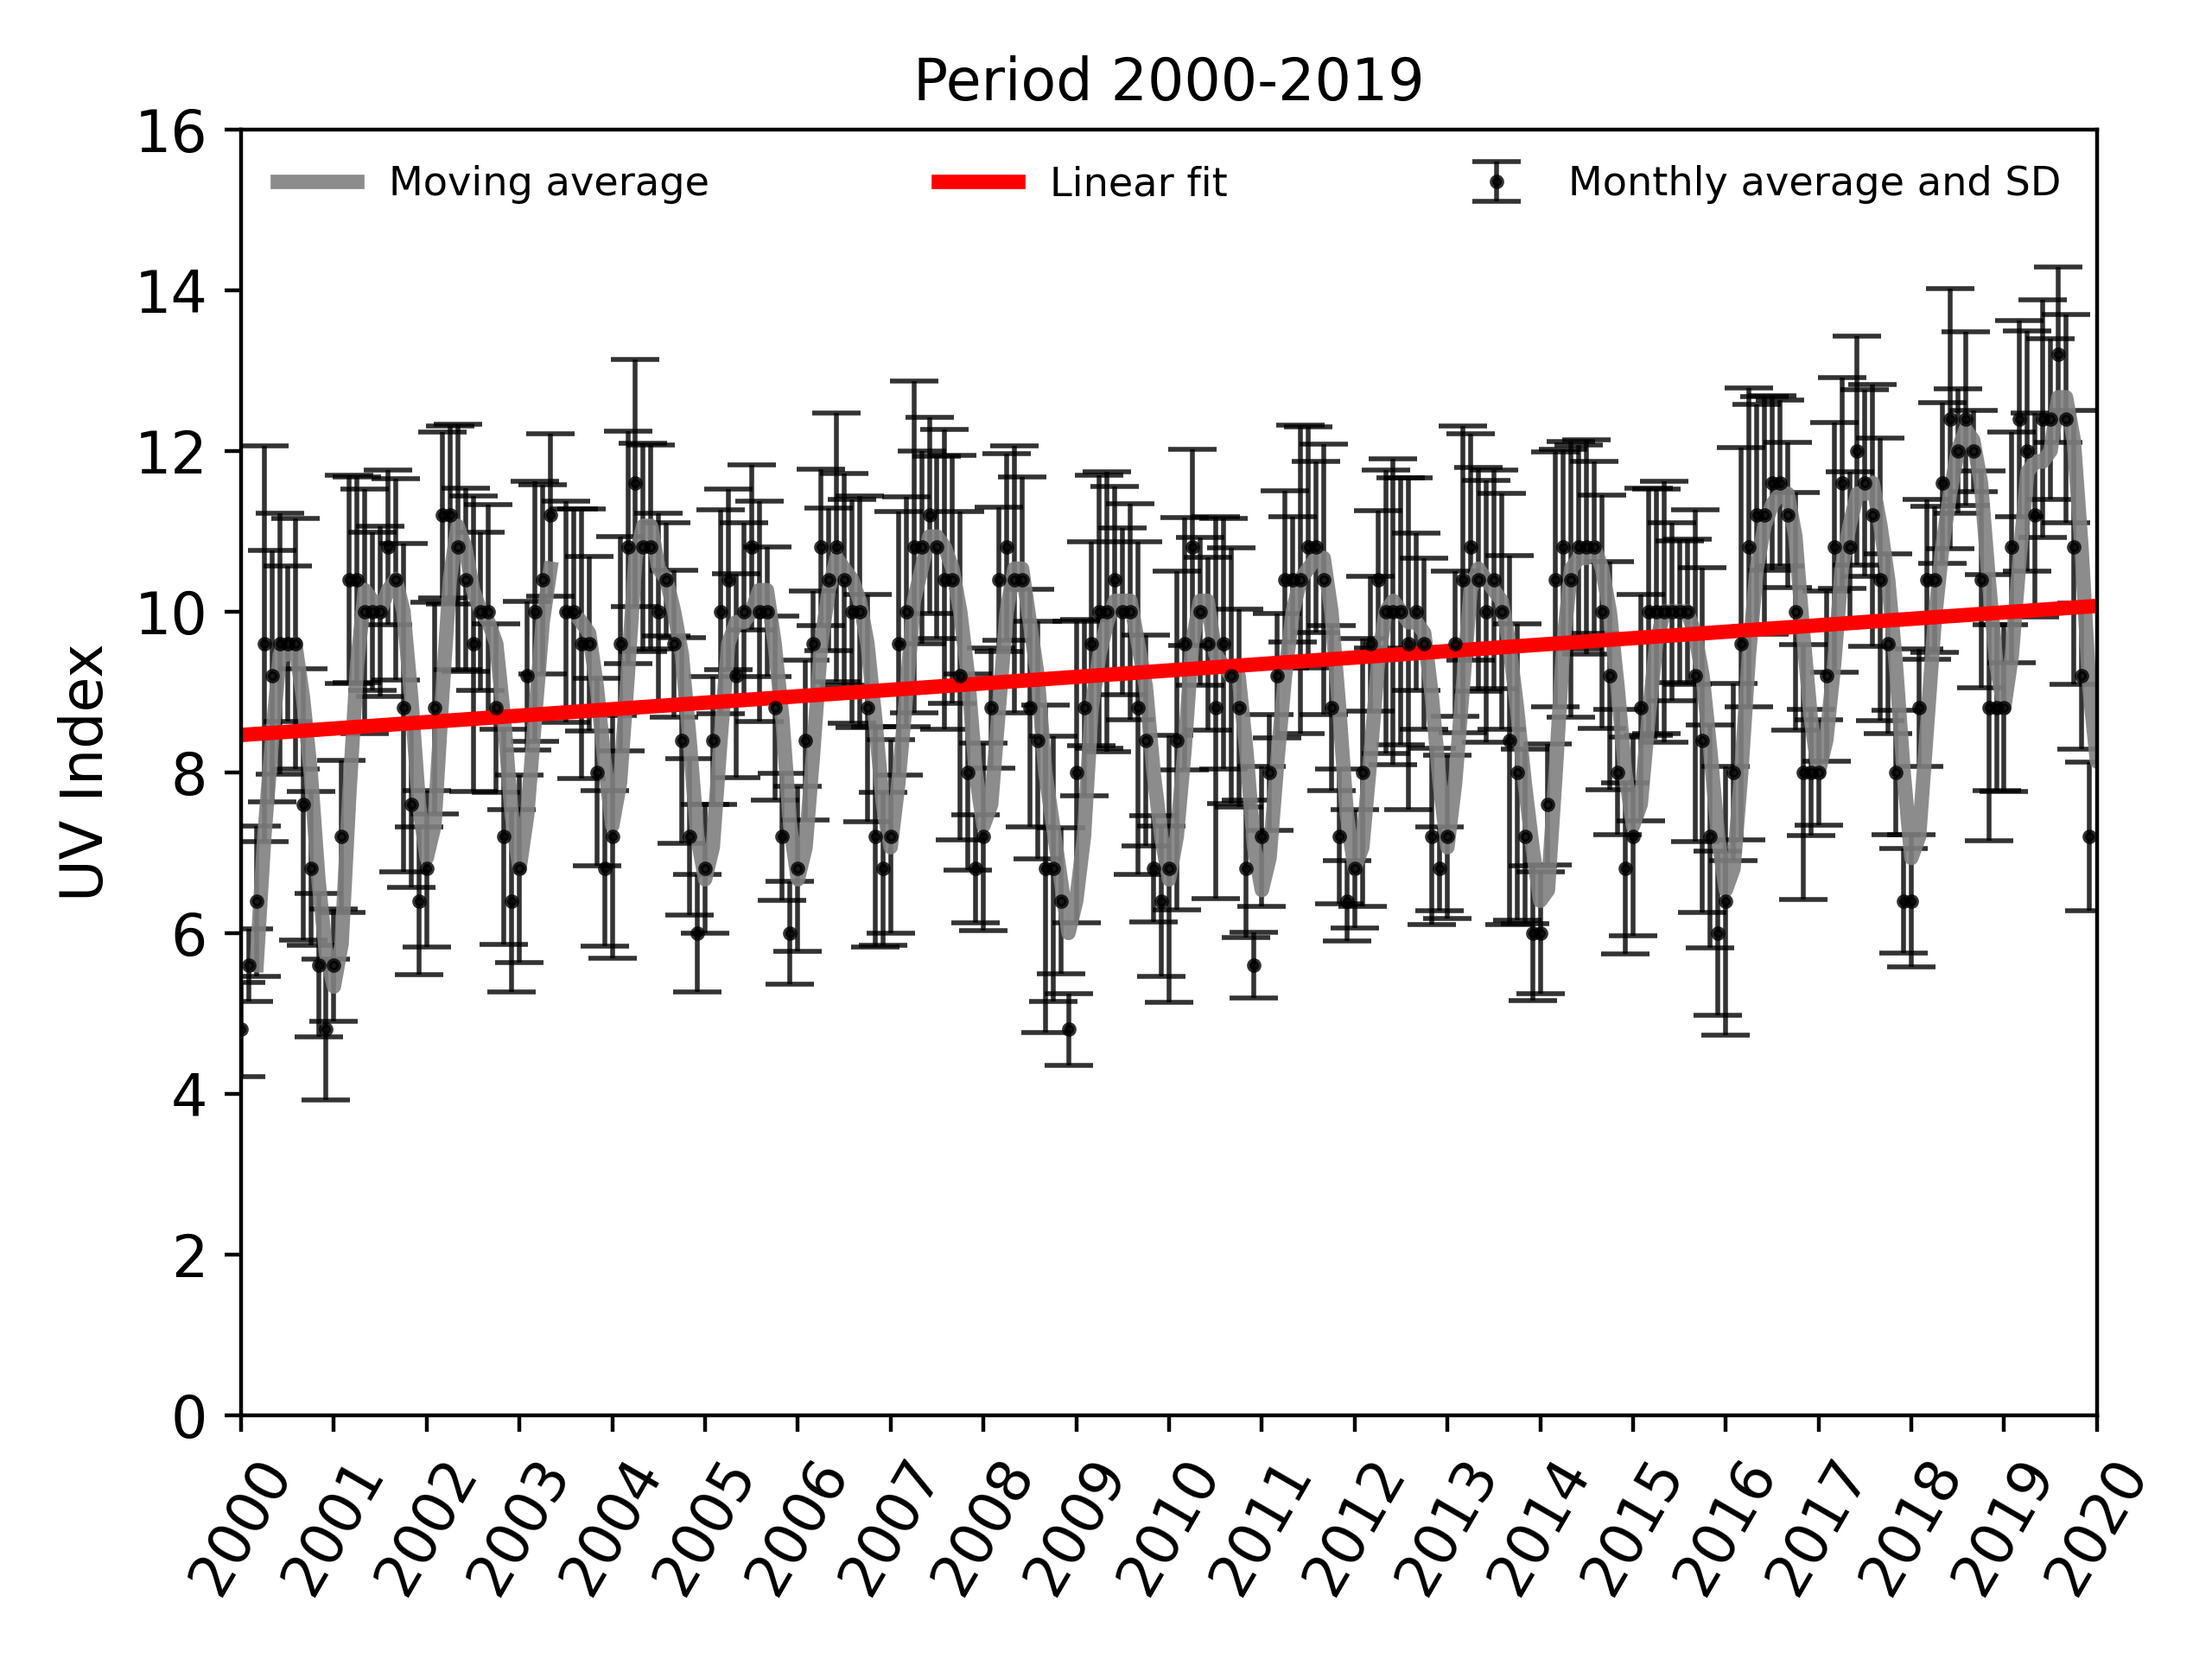
\includegraphics[width=0.70\columnwidth]{figures/UV_Moving_Average}
    \caption{{Moving average function (light gray curve) quarterly applied to monthly
          average UV Index, standard deviation of all data within a given month
          (black dots and dash line) and linear fit (red line).
            {\label{185758}}%
        }}
  \end{center}
\end{figure}

The UV Index computed from satellite-based observations
(OMI-Aura/NIVR-FMI-NASA) over the period 2005-2019 is mapped in
Figure~{\ref{485116}}. The satellite-derived UVIs vary
from 8 in winter to 16 in summer, both values being substantially higher
than the ground-based observations (ca. 7 for winter and 11 for summer,
see Fig.~{\ref{310112}}). We hypothesize that this
large difference between satellite-based estimation and ground-based
observation of the UV index is due to the intense air pollution of
Mexico City.~A rather similar behavior was detected in Santiago city,
Chile.\citep{Cabrera_2012}

Close inspection of Figure~{\ref{485116}} shows that
the maximum values, those from June and July of each year, show a slight
but systematic decrease starting ca. 2013. As mentioned in
section Methods, this is due to the post-processing of
OMI UVI data to account for absorption by BL aerosols\citep{Arola_2009},
using a climatological reduction of about 8\% for Mexico City.

\begin{figure}[H]
  \begin{center}
    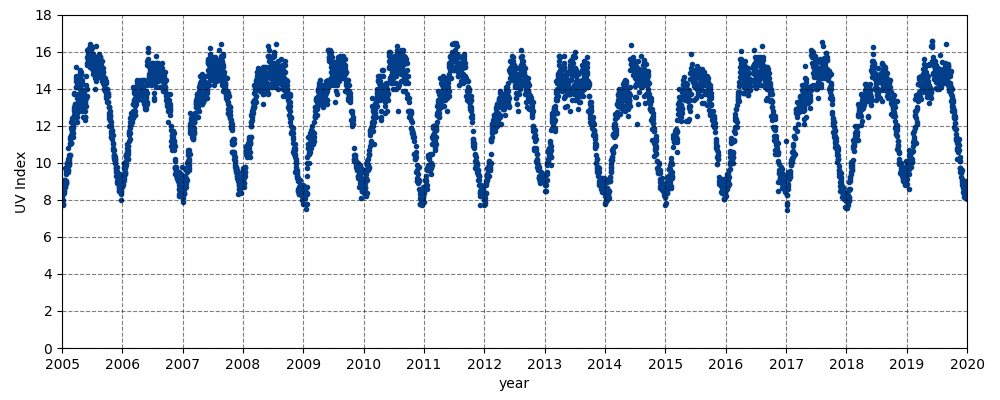
\includegraphics[width=0.70\columnwidth]{figures/CSUVindex}
    \caption{{UV Index at solar noon for clear sky recorded by OMI-Aura/NIVR-FMI-NASA,
          from 2005 to 2019.
            {\label{485116}}%
        }}
  \end{center}
\end{figure}


\subsection{Effect of pollutants on UV radiation}

Trends and averages in aerosol optical depth AOD\textsubscript{340} and
criteria pollutants PM\textsubscript{10}, CO, NO\textsubscript{2},
O\textsubscript{3~}and SO\textsubscript{2} observed at the SIMAT
stations over 2000-2019, are shown in
Figure~{\ref{829996}} and summarized in
Table~{\ref{table:uvindex}} together with
the~\(UVI_{\max}\). Similar trends in pollutants have been noted
before\citep{Parrish_2011,aire_cmdx_2017,Molina_2019}
and reflect the long-term success of
emission reduction policies and programs.

\begin{figure}[H]
  \begin{center}
    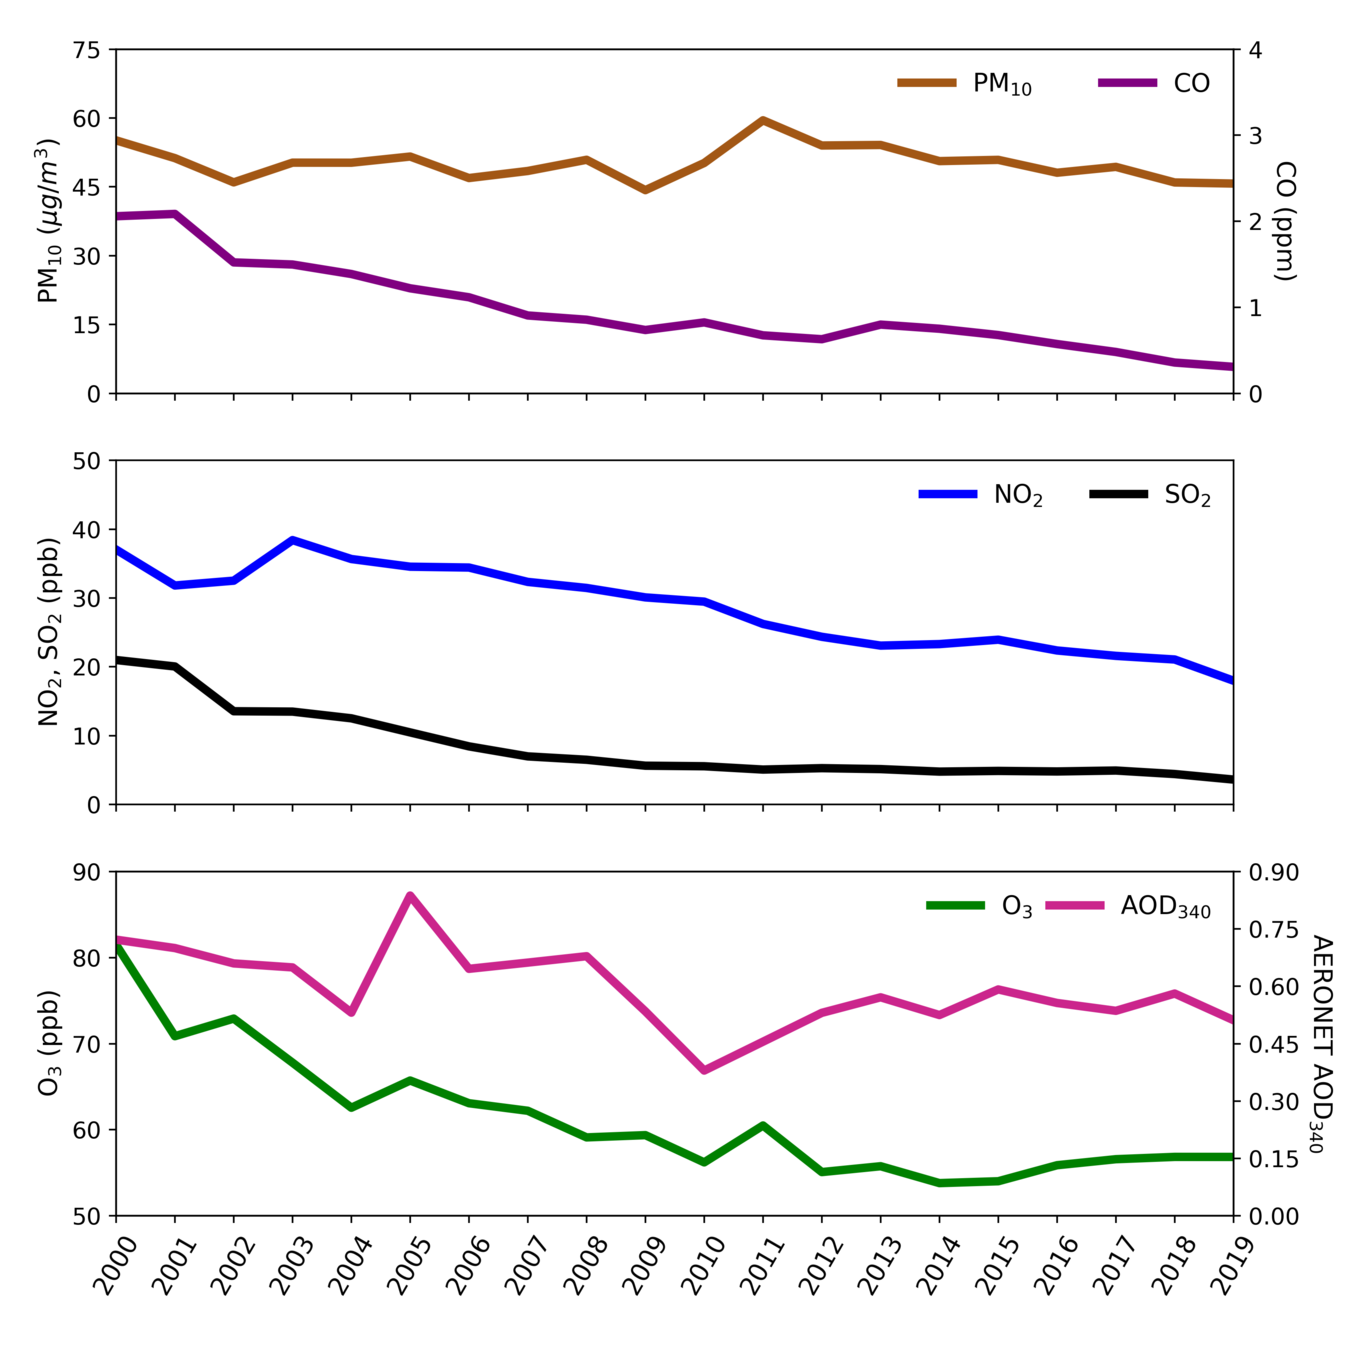
\includegraphics[width=0.63\columnwidth]{figures/pollutants}
    \caption{{Air quality trends in MCMA for the period 2000-2019~ from annual
    averages obtained between 11h to 15h CST every day: PM\textsubscript{10}
    (brown curve), CO (purple curve), NO\textsubscript{2} (blue curve),
    SO\textsubscript{2}(black curve), O\textsubscript{3} (green curve) and
    AOD\textsubscript{340} (pink curve).
    {\label{829996}}%
    }}
  \end{center}
\end{figure}

\begin{table}[H]
  \centering
  \begin{tabular}{cccc} \hline
    Variable               & $\frac{\Delta variable}{\Delta t}$ & Avg$_{2000-2019}$ & $\Delta(\%/year)$ \\ \hline
    UVI                    & 0.08                               & 9.2               & 0.9               \\
    PM\textsubscript{10}   & -0.10                              & 50.2              & -0.2              \\
    CO                     & -0.08                              & 1.0               & -8.2              \\
    NO\textsubscript{2}    & -0.96                              & 28.6              & -3.4              \\
    O\textsubscript{3}     & -1.05                              & 61.3              & -1.7              \\
    AOD\textsubscript{340} & -0.01                              & 0.6               & -1.6              \\
    SO\textsubscript{2}    & -0.76                              & 8.4               & -9.1              \\
    \hline
  \end{tabular}
  \caption{{{{UV Index and criteria pollutants: slope for the period 2000-2019,
                averages in units of $\mu g/m^3$(PM$_{10}$), ppm (CO), ppb
                (SO$_2$, NO$_2$ and O$_3$), dimensionless (UV Index and AOD$_{340}$) and
                annual percentage change (\%/year).}}}}
  \label{table:uvindex}
\end{table}

The observed changes in the concentrations of these air pollutants have
significant implications for surface UV radiation, as can be
demonstrated with the TUV radiative transfer model.
Table~{\ref{table:TUVmodel}} summarizes UVI values for
the June-July time period, estimated by the three methods: OMI
satellite-derived UVI, RAMA ground-based observations, and TUV modeling
using air pollution estimates. Two groups of values can be readily
identified: (1) RAMA daily record values, OMI with or without BL
aerosols, and TUV for very clean conditions, all with UVI values around
15-16; and (2) RAMA average daily maxima and TUV UVI using MCMA
pollutants as input, which are in good agreement for both 2018/19 and
2000/01 but much lower than the first group. Compared to the OMI
estimate that included the climatological aerosol correction (15.3),
observed RAMA values were lower by 35\% in 2000 and by 20\% in 2019.
Similarly, TUV values were 35\% lower in 2000 and 22\% lower in 2019
relative to the TUV values of 15.6 for a pristine atmosphere.

\begin{table}[H]
  \centering
  \begin{tabular}{lc}
    \hline
    \textbf{Conditions for estimation in June-July}                    & \textbf{UV Index} \\ \hline
    RAMA maximum reached in period 2000-2019                           & 15.0              \\ \hline
    RAMA average maxima 2018, 2019                                     & 12.3              \\ \hline
    RAMA average maxima 2000, 2001                                     & 9.9               \\ \hline
    OMI clear, local noon, no corrected for BL aerosols                & 16.6              \\ \hline
    OMI with 8\% reduction for BL aerosol (Figure 1 from Arola et al.) & 15.3              \\ \hline
    \begin{tabular}[c]{@{}l@{}}TUV "zero" pollution \\ AOD 0, O\textsubscript{3} 0 ppb, NO\textsubscript{2} 0 ppb, SO\textsubscript{2} 0 ppb\end{tabular}                                         & 16.1              \\ \hline
    \begin{tabular}[c]{@{}l@{}
      }TUV pristine pollution \\ AOD 0.05, O\textsubscript{3} 10 ppb, NO\textsubscript{2} 0 ppb, SO\textsubscript{2} 0 ppb\end{tabular}                                         & 15.6              \\ \hline
    \begin{tabular}[c]{@{}l@{}}TUV 2019:\\ AOD 0.5, O\textsubscript{3} 50 ppb, NO\textsubscript{2} 20 ppb, SO\textsubscript{2} 1 ppb\end{tabular}                                         & 12.1              \\ \hline
    \begin{tabular}[c]{@{}l@{}}TUV 2000:\\ AOD 0.7, O\textsubscript{3} 70 ppb, NO\textsubscript{2} 40 ppb, SO\textsubscript{2} 20 ppb\end{tabular}                                         & 10.2              \\ \hline
  \end{tabular}
  \caption{{UV Index monthly maximum estimates for June-July.}}
  \label{table:TUVmodel}
\end{table}

The agreement between RAMA observations and TUV model estimates is
excellent but also probably a bit fortuitous. Clouds on average reduce
the irradiance impingent on the surface, but scattering from them can
also cause transient enhancements (especially if the direct sunbeam is
not blocked) that could be recorded as daily maxima -- with cancellation
between these cloud effects resulting in improved agreement with the
cloud-free model. We cannot exclude that some of the observed trend in
UVI is due to changes in cloud cover. However, the modeled fractional
UVI reductions due to pollutants, shown in Table
  {\ref{table:TUVmodel}}, are in such good agreement with
the observed UVI reductions, that a compelling case can be made for a
dominant role of air pollutants in the long-term UVI trends.

Table~{\ref{table:year2000-2019}} shows the
contributions to UVI reductions from individual pollutants. Aerosols are
seen to be the major factor in both time periods, followed by
O\textsubscript{3}, NO\textsubscript{2}, and SO\textsubscript{2}. The
2000-2019 UVI increase is seen to result in comparable proportions from
fewer aerosols, less SO\textsubscript{2}, and the combined reductions in
O\textsubscript{3} and NO\textsubscript{2}.

Comparable UV reductions, of 30-40\% due to aerosols, were reported by
\citet{Panicker_2009} over Pune, India from April 2004 to
March 2005, with sensitivity coefficients (i.e. change in UVI per unit
change in AOD) similar to those found here in Table~\ref{table:TUVmodel}.

Comparisons of OMI with ground-based UV measurements have been reviewed
recently by \citet{Zhang_2019} and \citet{Vitt_2020}.
OMI-derived UV generally overestimates
ground-level measurements by 1-10\% in relatively clean conditions (e.g.
rural U.S), by 10-30\% in Southern Europe and by 40\% or more in
Santiago, Chile\citep{Cabrera_2012} and Thailand\citep{Janjai_2013}. The
overestimations appear related in large part to incomplete accounting of
UV absorption by BL aerosol, although other factors such as the
correction to solar noon may also introduce some
bias.\citep{Zhang_2019} Over Europe, ground-based UVI observations for
several decades are systematically lower than those estimated from
satellites even after consideration of climatological aerosol
distributions, showing the importance of local pollution not resolved
from space.\citep{Vitt_2020} However, difference between
satellite-derived and ground-based UVI was less than 1.0 UVI units in
over 90\% of the cases, in contrast to the difference of 3-5 units found
for Mexico City (Table~{\ref{461017}}).

UV reductions by air pollutants are expected to be most severe near the
surface, while chemical reactions leading to photochemical smog occur
through the vertical extent of the BL.
Figure~{\ref{973680}} shows the vertical profiles of
photolysis coefficients (the reciprocals of photolytic lifetimes) for
two key reactions, the photolysis of O\textsubscript{3} to yield excited
oxygen atoms O(1D), and the photolysis of NO\textsubscript{2}. In the
absence of optically active pollutants, these coefficients would be
nearly independent of altitude in the BL. However, the presence of
pollutants leads to a strong decrease toward the surface, with notably
more severe reductions in 2000 compared to 2019.~While the specific
values shown in the figure are only illustrative for typical conditions,
routine daily air quality modeling should carefully account for the long
term variations in these photolysis coefficients.


\begin{figure}[H]
  \begin{center}
    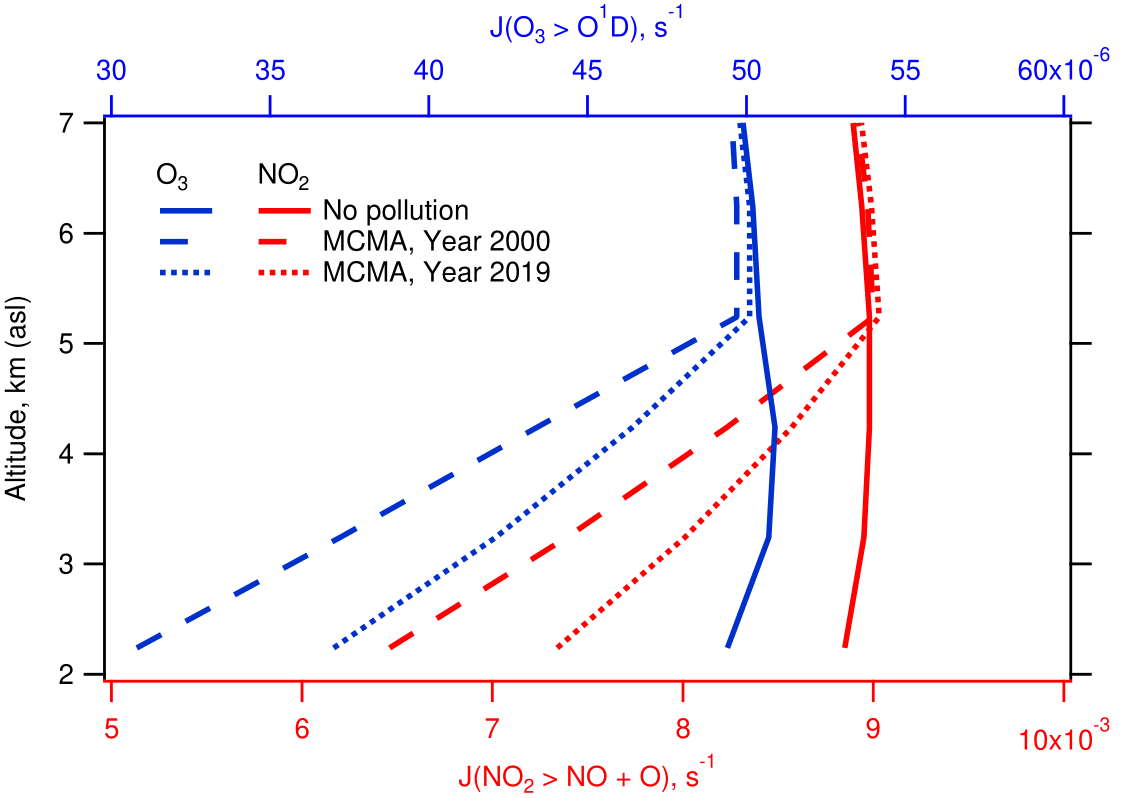
\includegraphics[width=0.70\columnwidth]{figures/jvals}
    \caption{{Vertical profiles of the photolysis coefficients for the
          reaction~\(O_3 + h\nu \rightarrow O(1D) + O_2\) (top axis, blue)~\(NO_2 + h\nu \rightarrow O+NO \) (bottom
          axis, red) for zero pollution (solid) and Mexico City in the years 2000
          (dashed) and 2019 (dotted)
          {\label{973680}}%
        }}
  \end{center}
\end{figure}

An issue that is beginning to gain relevance in radiative balance models
is the influence of a group of organic compounds capable of strongly
absorbing in the UV region (brown carbon).\citep{Laskin_2015} Some of
these compounds are related with emissions from local and regional
wildfires.\citep{Gadhavi_2010} Mexico City is frequently exposed to
regional fire smoke transport during the dry part of the year (November
to May)\citep{Rios_2019}, that sporadically modify the optical
properties of the aerosols.\citep{Barnard_2008} This could partly explain
the relatively minor reductions in PM\textsubscript{10} (see
Fig.~{\ref{829996}}), compared to the larger reductions
of CO, NO\textsubscript{2}, and O\textsubscript{3} that are more
directly related to urban activities, as well as some of the seasonal
asymmetry seen in Fig. {\ref{461017}}. ~

The UVI is specific to wavelengths mainly in the 300-320 nm range, and
so the question remains whether these results can be applied at longer
UV wavelengths, e.g. those important for NO\textsubscript{2} photolysis
(\textless{}420 nm). Absorption by SO\textsubscript{2} and
O\textsubscript{3} vanishes, while absorption by NO\textsubscript{2}
increases and typical aerosols optical depth decrease. These changes can
easily be modeled, but unfortunately far fewer measurements of these
longer wavelengths are available in Mexico City or elsewhere.

Two decades of observations in Mexico City demonstrate unequivocally
that air pollution reduces UV radiation at the ground. The ground-based
observations are well below estimates derived from satellite-based
observations, and below model calculations do not consider optically
important pollutant aerosols, tropospheric ozone, and to a lesser extent
NO\textsubscript{2} and SO\textsubscript{2}. When typical observed
values of these pollutants are included in a model (e.g. TUV), the
differences between satellite-derived and ground-based measured values
are explained and can be attributed quantitatively to individual
observed pollutants. Long term improvements in air quality, over two
decades, are accompanied by statistically significant increases in the
observed UVI, again in good agreement with the model-predicted changes.


\begin{table}[H]
  \centering
  \begin{tabular}{lccccc}
    \hline
    \multicolumn{1}{c}{\multirow{2}{*}{Pollutant}} & \multicolumn{2}{c}{Year 2000} & \multicolumn{2}{c}{Year 2019} & 2019-2000                 \\ \cline{2-6}
    \multicolumn{1}{c}{}                           & poll. level (a)               & UVI (b)                       & poll. level & UVI   & (c) \\ \hline
    AOD                                            & 0.7                           & -3.7                          & 0.5         & -2.7  & 1.0 \\
    O\textsubscript{3} ppb (DU)                    & 70 (14)                       & -1.4                          & 50 (10)     & -1.0  & 0.4 \\
    NO\textsubscript{2} ppb                        & 40                            & -0.9                          & 20          & -0.5  & 0.4 \\
    SO\textsubscript{2} ppb                        & 30                            & -0.8                          & 1           & -0.04 & 0.8 \\ \hline
  \end{tabular}
  \caption{Contributions of individual pollutants to UV Index changes. (a) Values used one at the time, with the others held at zero. (b) UVI deviation from the zero-pollution value of 16.1 (from Table \ref{table:TUVmodel}). (c) 2019-2000 UVI change due to changes in each pollutant.}
  \label{table:year2000-2019}
\end{table}

The reductions in surface UV radiation with respect to an ideally clear
atmosphere -- by nearly 40\% in 2000 and still 20\% in 2020 -- are
large, both within the context of human UV exposure and air quality
mitigation. In urban areas where ozone production scales proportionally
with UV levels and with volatile organic compound~(VOC) emissions (the
VOC-limited regime), a 10\% increase in BL average photolysis rates
means that VOC emissions will need to be reduced by 10\% to meet the
same goals, or else successful reductions in aerosols would lead to
unwanted UV-driven increases in O\textsubscript{3}.~Such UV changes must
be considered carefully in air quality mitigation strategies. For human
exposure, a 20\% increase in UV irradiances over two decades should be
seen as a non-negligible public health issue requiring some reassessment
of preventive behaviors to minimize the risk of skin cancer, cataract,
and other UV-related health effects. The efforts that Mexico City has
made to improve air quality have achieved positive results in the levels
of most air pollutants. Nevertheless, they caused an increase in UV
radiation that reaches the surface.

A limitation of the present work is our focus on daily maximum values,
which largely exclude cloud cover. Absorption within clouds can be
enhanced by the long path lengths of multiply scattered photons (e.g.,
\citet{Mayer_1998}), so that accurate quantification of UV
effects of clouds in polluted environments remains a significant
challenge and interesting opportunity for future work.







%%%%%%%%%%%%%%%%%%%%%%%%%%%%%%%%%%%%%%%%%%%%%%%%%%%%%%%%%%%%%%%%%%%%%
%% The "Acknowledgement" section can be given in all manuscript
%% classes.  This should be given within the "acknowledgement"
%% environment, which will make the correct section or running title.
%%%%%%%%%%%%%%%%%%%%%%%%%%%%%%%%%%%%%%%%%%%%%%%%%%%%%%%%%%%%%%%%%%%%%
\begin{acknowledgement}
  We wish to acknowledge the staff of SIMAT, from the Secretariat of
  Environment, for the data and the continuous assistance during the
  realization of this project. Adriana Ipiña would like to extend her
  thanks to Dirección General de Personal Académico, Universidad
  Nacional Autónoma de México (DGAPA-UNAM) for the postdoctoral fellowship
  at Centro de Ciencias de la Atmósfera of the UNAM. Rubén D Piacentini
  wishes to thank CONICET and National University of Rosario, Argentina,
  for their partial support to the present work. The National Center for
  Atmospheric Research is sponsored by the National Science Foundation.
\end{acknowledgement}



% %%%%%%%%%%%%%%%%%%%%%%%%%%%%%%%%%%%%%%%%%%%%%%%%%%%%%%%%%%%%%%%%%%%%%
% %% The same is true for Supporting Information, which should use the
% %% suppinfo environment.
% %%%%%%%%%%%%%%%%%%%%%%%%%%%%%%%%%%%%%%%%%%%%%%%%%%%%%%%%%%%%%%%%%%%%%
% \begin{suppinfo}

% A listing of the contents of each file supplied as Supporting Information
% should be included. For instructions on what should be included in the
% Supporting Information as well as how to prepare this material for
% publications, refer to the journal's Instructions for Authors.

% The following files are available free of charge.
% \begin{itemize}
%   \item Filename: brief description
%   \item Filename: brief description
% \end{itemize}

% \end{suppinfo}



%%%%%%%%%%%%%%%%%%%%%%%%%%%%%%%%%%%%%%%%%%%%%%%%%%%%%%%%%%%%%%%%%%%%%
%% The appropriate \bibliography command should be placed here.
%% Notice that the class file automatically sets \bibliographystyle
%% and also names the section correctly.
%%%%%%%%%%%%%%%%%%%%%%%%%%%%%%%%%%%%%%%%%%%%%%%%%%%%%%%%%%%%%%%%%%%%%
\bibliography{bibliography/bibliodoi}

\end{document}
